% Copyright (c) 2014,2016 Casper Ti. Vector
% Public domain.

\chapter{HybriG系统设计} \label{chap:design}
\section{HybriG的系统架构概述}
为了更好地应对含有大量重边的属性图应用场景,规避传统图数据库的局限性,本文提出了一种复合存储架构HybriG。
HybriG将图的连接信息和点集的属性数据存储在Titan中,边集的所有属性数据则直接存储在HBase中。由于HybriG架构基于Titan和 HBase实现存储,而Titan的数据本身也存储在HBase中,为了方便表述以及避免混淆,下文中的HBase指的都是不包含Titan数据表的部分。Titan在HBase中的数据表直接用 Titan 代称。

\begin{figure}[htbp]
\centering
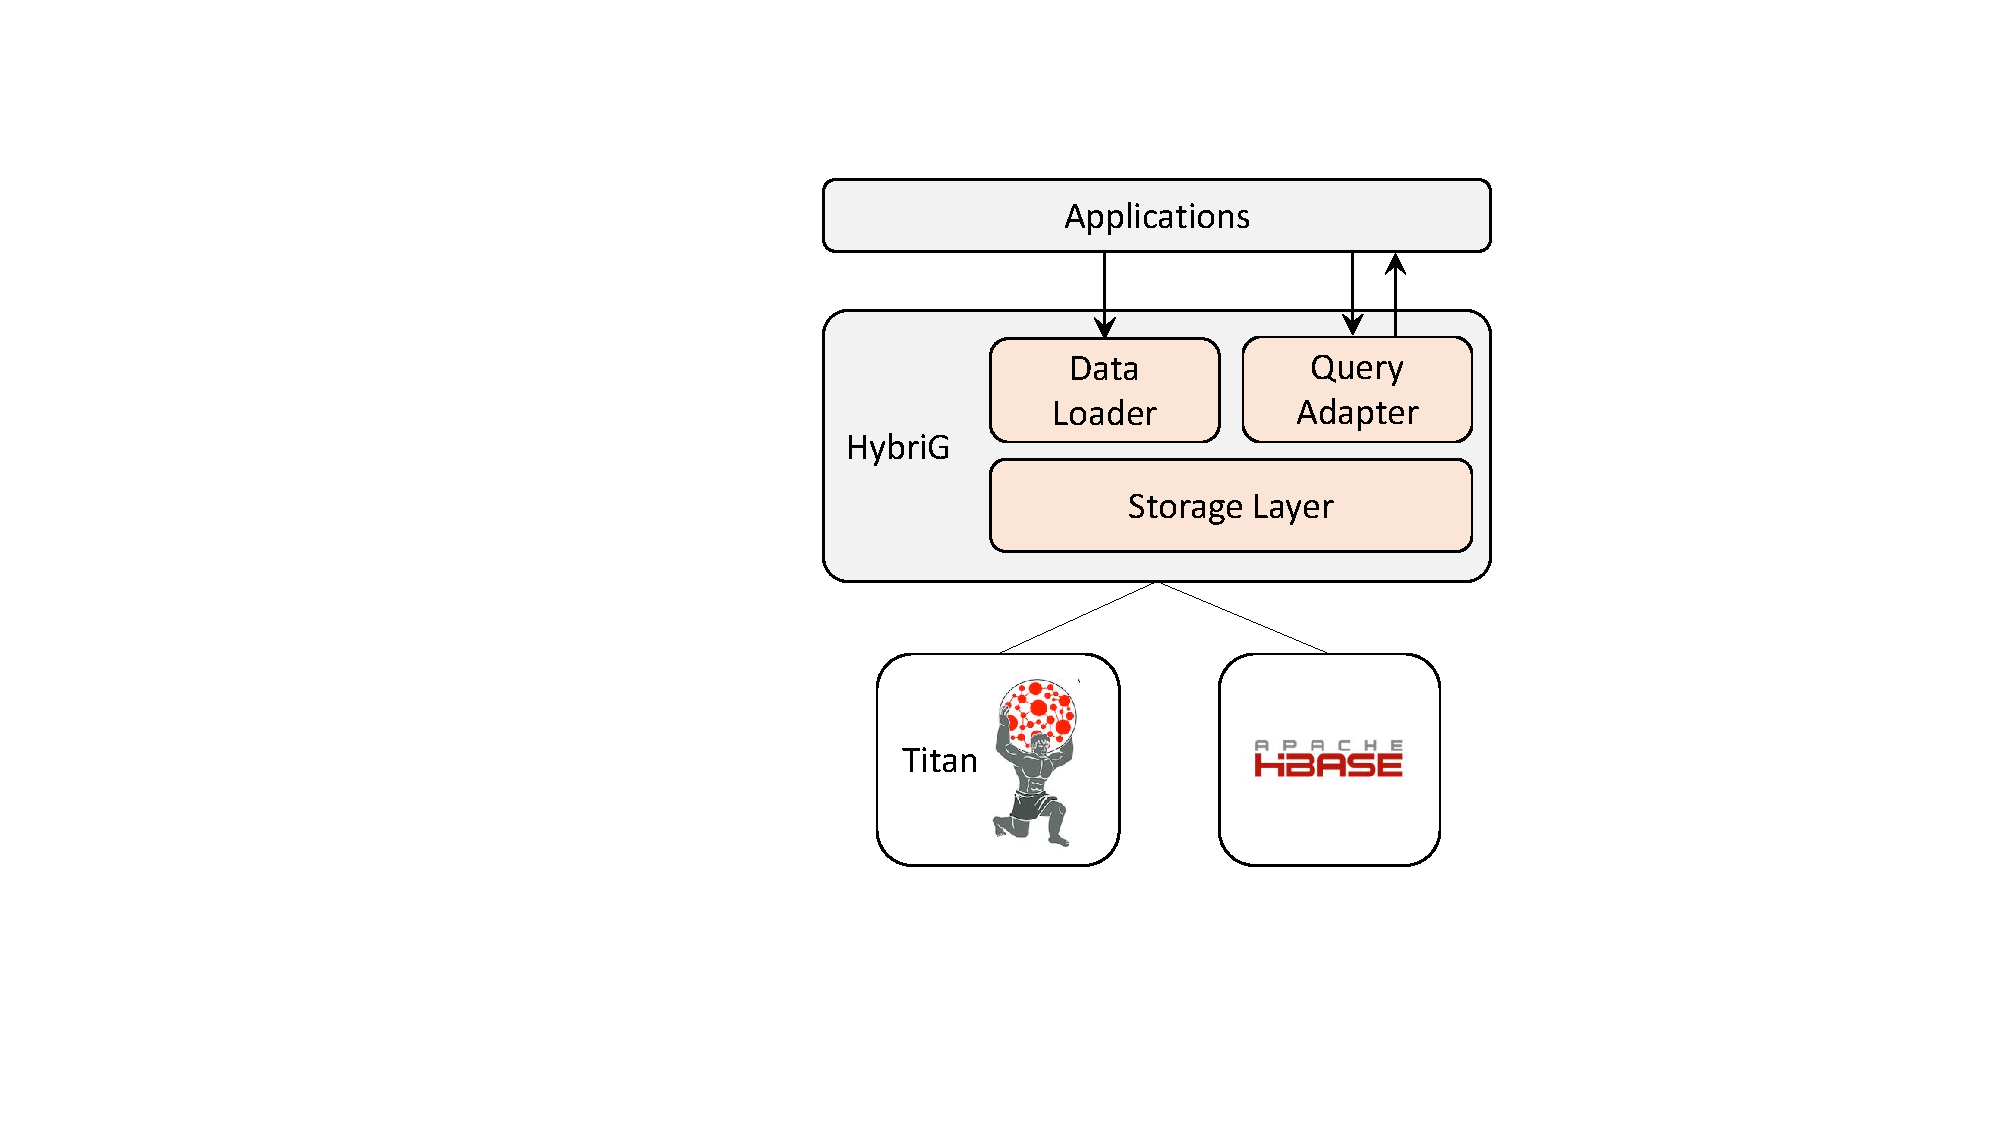
\includegraphics[height=80mm]{fig/arch.pdf}
\caption{HybriG系统架构}
\label{fig:arch}
\end{figure}

图 \ref{fig:arch}展示了HybriG的系统架构。Storage Layer是HybriG的存储层,Query Adapter和 Data Loader分别为用户程序提供图查询和数据插入接口。其中,Query Adapter将图查询转换为对Titan和HBase数据的高效查询,再将结果汇总返回给用户程序。Data Loader实现了数据的高效导入,在面对大批量的数据导入时,实现了错误恢复、断点恢复机制,同时保证了Titan和HBase的数据一致性。下面将分别介绍HybriG各模块的实现。


\section{Storage Layer}
HybriG将图数据分开存储在Titan和HBase中。具体地,如果两点之间有相同label的重边,HybriG会在Titan中这两点间建立一条该label的边,将对应重边的数据都存储在HBase中的一个表,不妨称其为边表。每条边一行,行键是Titan图中分配的边id拼接上重边的主键,单元格的值则存放具体边的内容。重边的主键是这样定义的:在两点间同label的重边中,如果有一个属性能唯一确定一条边,则选该属性作为主键。比如交易关系的时间戳,两个人在同一个时间点只能发生一次交易,因此该时间戳可以唯一确定两人间的一次交易。如果某种label的边没有属性能唯一确定一条重边,则选该数据插入的时间戳作为主键。

在HBase边表中,同label的重边数据的行键都有相同的前缀(即Titan中的边id),由于HBase中的数据是按行键排序的,它们在HBase中有相邻的位置。同label的重边经常会被同时检索,这种设计使得一次顺序扫描便可得到所有同label的重边。另外,HybriG利用Titan中边上的属性记录一些统计信息,如原图中实际有几条这样的重边,或者边上某个属性值的求和等,这些统计信息可以根据业务定制,用来加快业务相关的查询,不用再遍历相关的边。

\begin{figure}[htbp]
\centering
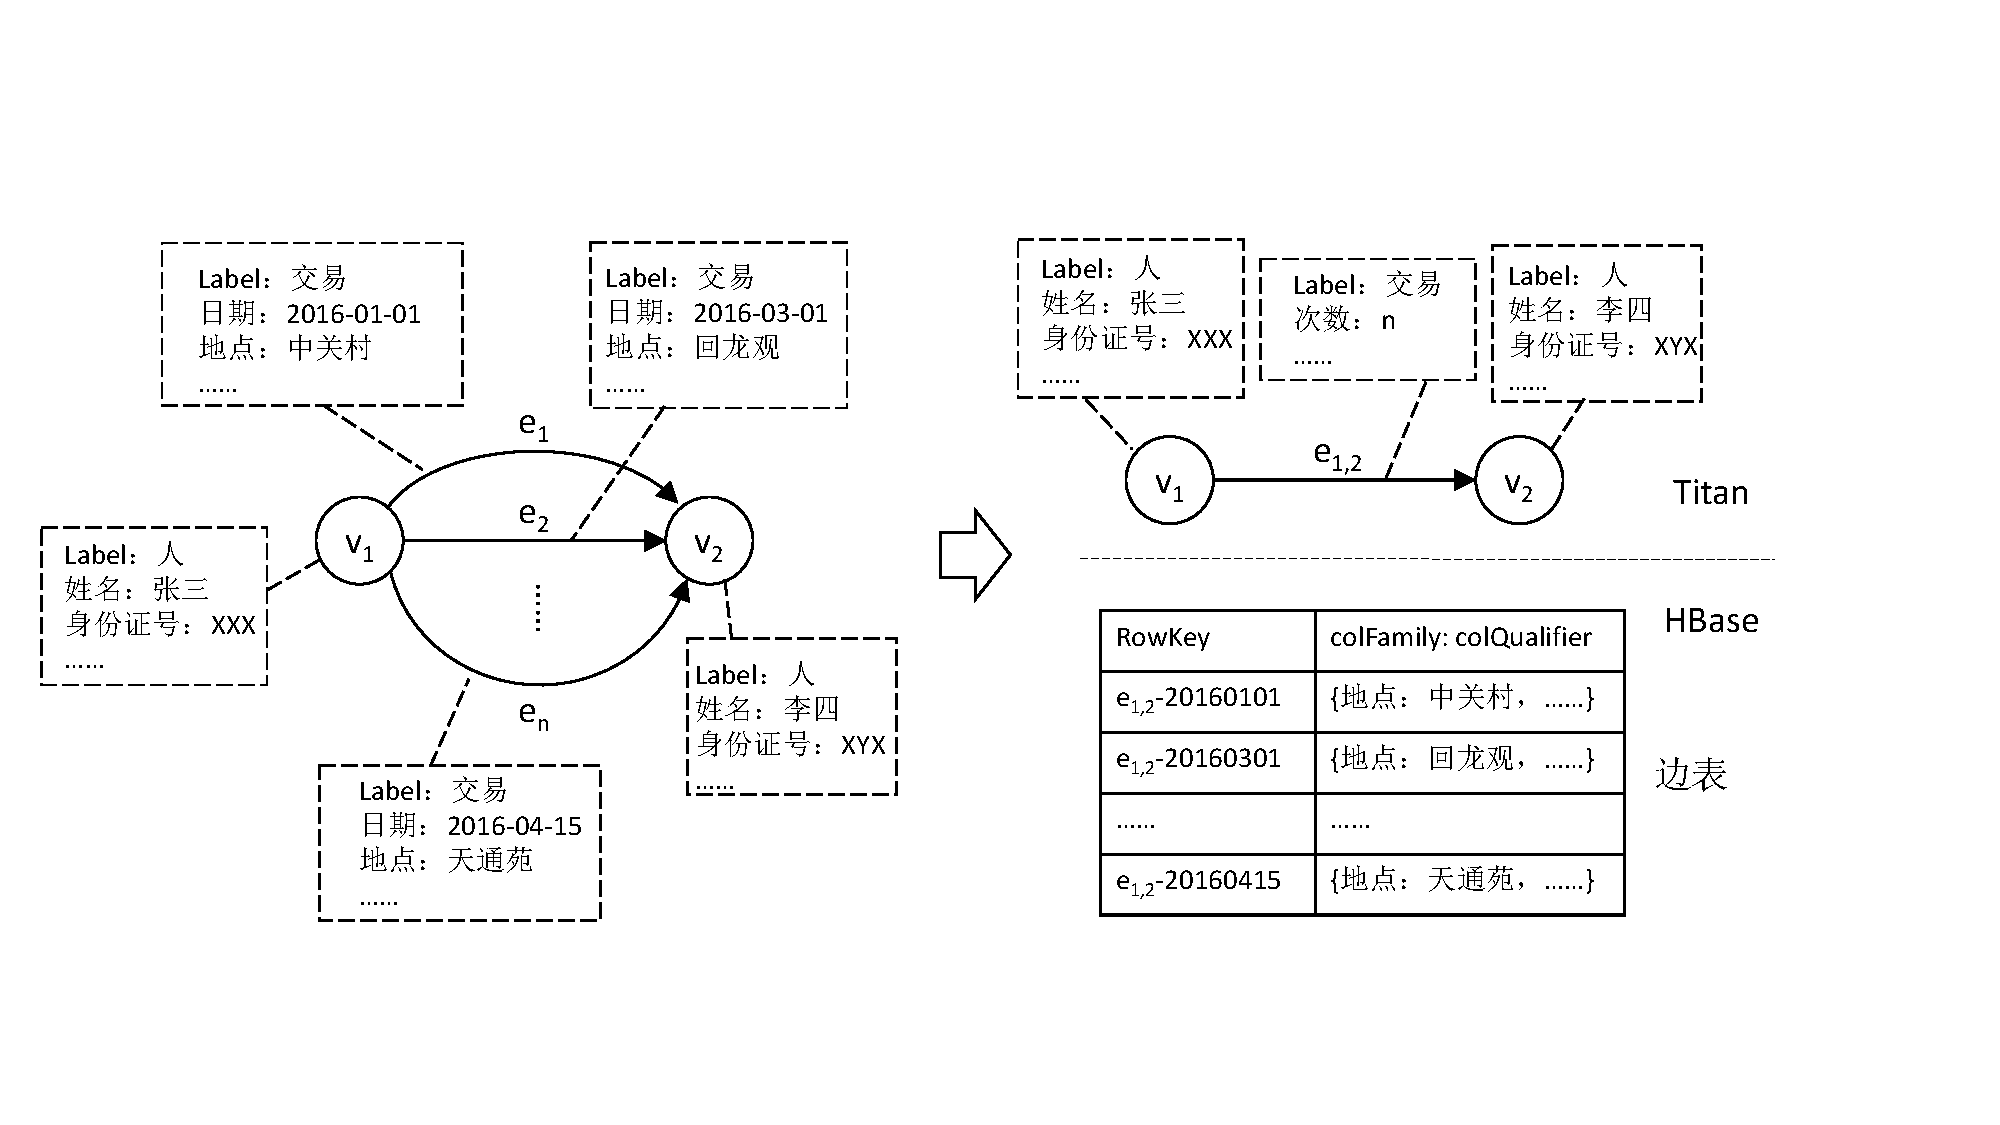
\includegraphics[width=150mm]{fig/storage_layer.pdf}
\caption[HybriG存储示例]{HybriG存储示例。左图为原始数据的属性图,右图为数据在Titan和HBase边表的存储情况。}
\label{fig:storage_layer}
\end{figure}

图 \ref{fig:storage_layer}是数据存储的一个示例,左边是实际要存储的图数据, e1、e2、…、en都是label为“交易”的重边,表示两人的所有交易记录。右边是数据在Titan和HBase中的存储情况。Titan中只存一条label为“交易”的边,该边有一个属性记录实际的边数。利用这条边的id作为前缀,拼接上重边的主键(交易的时间戳)作为HBase的行键,将每条边的数据都存入对应的单元格中。

本文在引言中提到了一种避免产生重边的建模方式,即将所有同label的重边合并为一条边来表示,边上存储这些重边的所有数据。HybriG架构与其有相似之处,但本质区别是边集元素的数据粒度仍是每条重边,不会将多条重边的数据作为一个单元来处理。在HybriG中每条边的数据独占HBase边表中的一行,因此每条边的相关操作都会更加高效。得益于HBase的高可扩展性,这种存储方式的性能也不会受制于数据规模的增长。而前述建模方式将所有重边的数据合并在一条边中存储,当重边量级巨大时,对每条边的操作势必更加低效。

\begin{figure}[htbp]
\centering
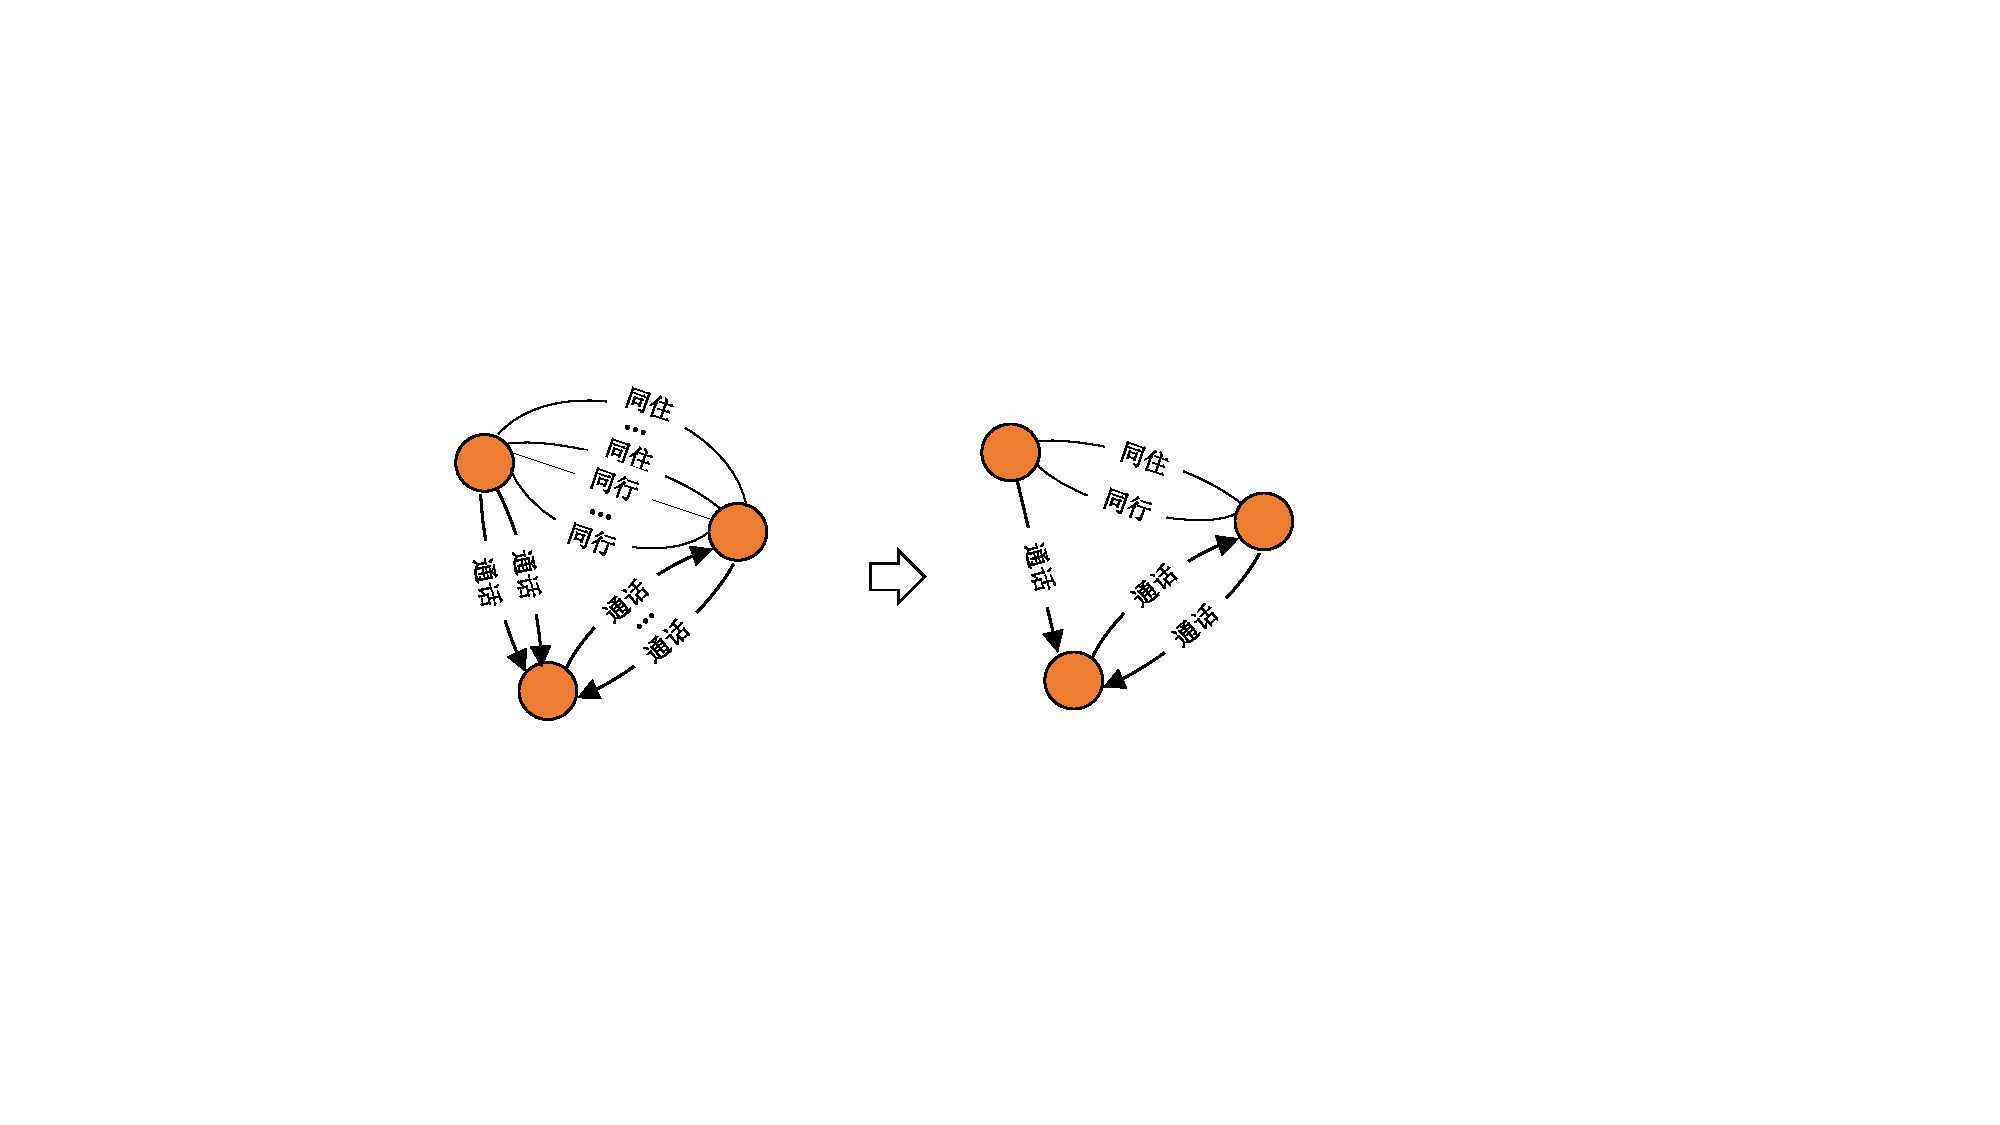
\includegraphics[width=100mm]{fig/merge_edges.pdf}
\caption[合并同label重边示意图]{合并同label重边示意。左图为实际数据图,右图为Titan中的存储示意图。无向边中的重边是指端点对应相同的两条或多条边,有向边中的重边是指起点和终点对应相同的两条或多条边。}
\label{fig:merge_edges}
\end{figure}

HybriG采用的是合并同label的重边,而不是所有的重边,这仍是基于数据粒度的考虑。图\ref{fig:merge_edges}是合并相同label重边后Titan的图示例(在HBase边表中的重边数据未显示)。在实际应用场景中,经常需要根据具体的关系种类(label)来进行邻域点集查找,对于具体边数据的查询也常按label进行。因此合并相同label的重边设计可以使很多查询在Titan中就得到满足,不需要再涉及HBase边表。


\section{Query Adapter}
Query Adapter模块将图查询转化为对应Titan和HBase的查询,再将结果汇总返回。下面分别叙述其查询设计、查询实现以及查询优势。
\subsection{查询设计}
我们在HybriG架构上实现了基本图查询接口,暴露给上层应用的仍是一张属性图。基本的图查询接口可分为如下几类:
\begin{itemize}
	\item 以点为中心的查询:获取某点邻接的点、获取某点的属性、获取某点邻接的边等;
	\item 以边为中心的查询:获取某条边的端点、获取某条边的属性等;
	\item 从图中直接查询:查询符合某种条件的元素(点/边),其中的条件可以是label、限定返回集大小(limit)等。
\end{itemize}
更详细的属性图查询接口,可以查看Blueprints中的定义。

除了基本的属性图查询接口,HybriG还提供了重边的统计信息查询。比如查询两点间某种label的重边具体的边数、或者查询某个属性上的聚集信息(如MIN、MAX、AVG、SUM等),可以根据业务需要来定制具体统计的信息。比如通话关系所表示的边中,有记录通话开始时间戳的属性。可以设置HybriG统计该类重边在该属性的最小值,从而可以查询两人最早的通话发生时间。在HybriG架构中,这些统计信息存储在Titan中的边上,因而可以快速返回结果,无需再对具体的边数据(存在HBase边表中)进行统计。

区别于传统Titan图数据库,我们没有实现事务性的接口,如newTransaction、 commit 和 rollback 等。因为业务场景可以规避对事务性的依赖,在富含重边的应用场景中,边集数据都是事件记录类型的数据,数据导入后就无需修改。而且数据导入可以分批定期执行,不会有多数据源写入导致的写-写冲突或读-写冲突。另外HybriG的数据分开存储在Titan和HBase两个数据库中,实现严格事务的代价比较大,会带来显著的性能牺牲。如Google的 Percolator\supercite{percolator} 在 BigTable 上实现了分布式事务,但写性能有75\%的牺牲。

\subsection{查询实现}
查询的实现可分为两部分,一部分只依赖于Titan中的数据,另一部分需要联合Titan 和 HBase边表的数据来返回结果。下面分别叙述。
\subsubsection{仅依赖Titan数据的查询}
在HybriG架构中,点集和各点的邻接信息都存储在Titan中,因此只与点集相关的查询都可以直接转换为对Titan的查询,如点上属性的查询、查询给定点的邻域点集、在图中查询某种label的点等。

对于重边的统计信息查询,其需要的统计结果都已在Titan的边中存储,故可以直接转换为对Titan边上的属性值查询。具体实现中需要维护一个映射关系作为元信息,以得知一个统计信息对应Titan边上的哪个属性。
\subsubsection{关联Titan和HBase数据的查询}
当查询具体的边数据时,就需要关联Titan和HBase来实现查询。在HybriG架构中,
$$HybriG\_Edge = TitanEdgeID + HBaseRowData$$
上式表示每条边对象的两部分组成,所有边集数据存储在HBase的边表中,每条边的数据占据一行,存储其所有属性,该行的行键是Titan中对应的边id拼接上该边的主键值。因此查询某条重边的数据,需要先在Titan中找到对应边的id,再在HBase边表中找到对应行的数据。

下面以两点间边集查询为例阐述HybriG的实现。两点间边集查询是指给定两个点,查询它们之间满足某种条件的边。比如已经从邻域查询得知v1与v2相邻,现在想得到它们之间某种label的所有边。查询的伪代码见算法\ref{alg:edge_query}.
\begin{algorithm}
\caption{两点间给定label的边集数据查询伪代码}
\label{alg:edge_query}
\begin{algorithmic}[1] % 每1行显示一个行号
\REQUIRE 点v1,点v2,eLabel
\ENSURE 两点间的所有符合条件的边集数据

\STATE e = v1.query().adjacent(v2).label(eLabel)
.limit(1).edges().next()
\IF{e == null}
\RETURN null
\ENDIF
\STATE res = hbaseTable.scan(e.id, next(e.id))
\RETURN wrapEdges(res)
\end{algorithmic}
\end{algorithm}

算法\ref{alg:edge_query}中,第1行查询两点间该label的边,并利用limit(1)修饰来加速,在HybriG架构中,Titan只在这两点间存储该label的一条边,因此我们可以利用边的唯一性来加速查询。第2-4行,若在Titan中查询到该label的边不存在,则不需要再在HBase中检索。第5行根据Titan中的边id,在HBase的边表中通过Scan查询得到所有边的具体数据。e.id是一个字符串,伪代码中的next(e.id)表示同等长度的下一个字符串,即将字符串e.id中最后一个字符的值加一。比如e.id为“abbb”,则next(e.id)为“abbc”。HBase的Scan函数返回连续的若干行数据,接收的两个参数是行键范围的起始和结束点,是一个左开右闭的区间。用e.id和next(e.id)作为该区间的左右端点,即可查询到所有行键以e.id作为前缀的数据。最后第6行wrapEdges函数将这些数据转换为具体的边对象,每行一条边。

\subsection{HybriG的查询优势}
\subsubsection{邻域点集相关查询的优势}

\begin{figure}[htbp]
\centering
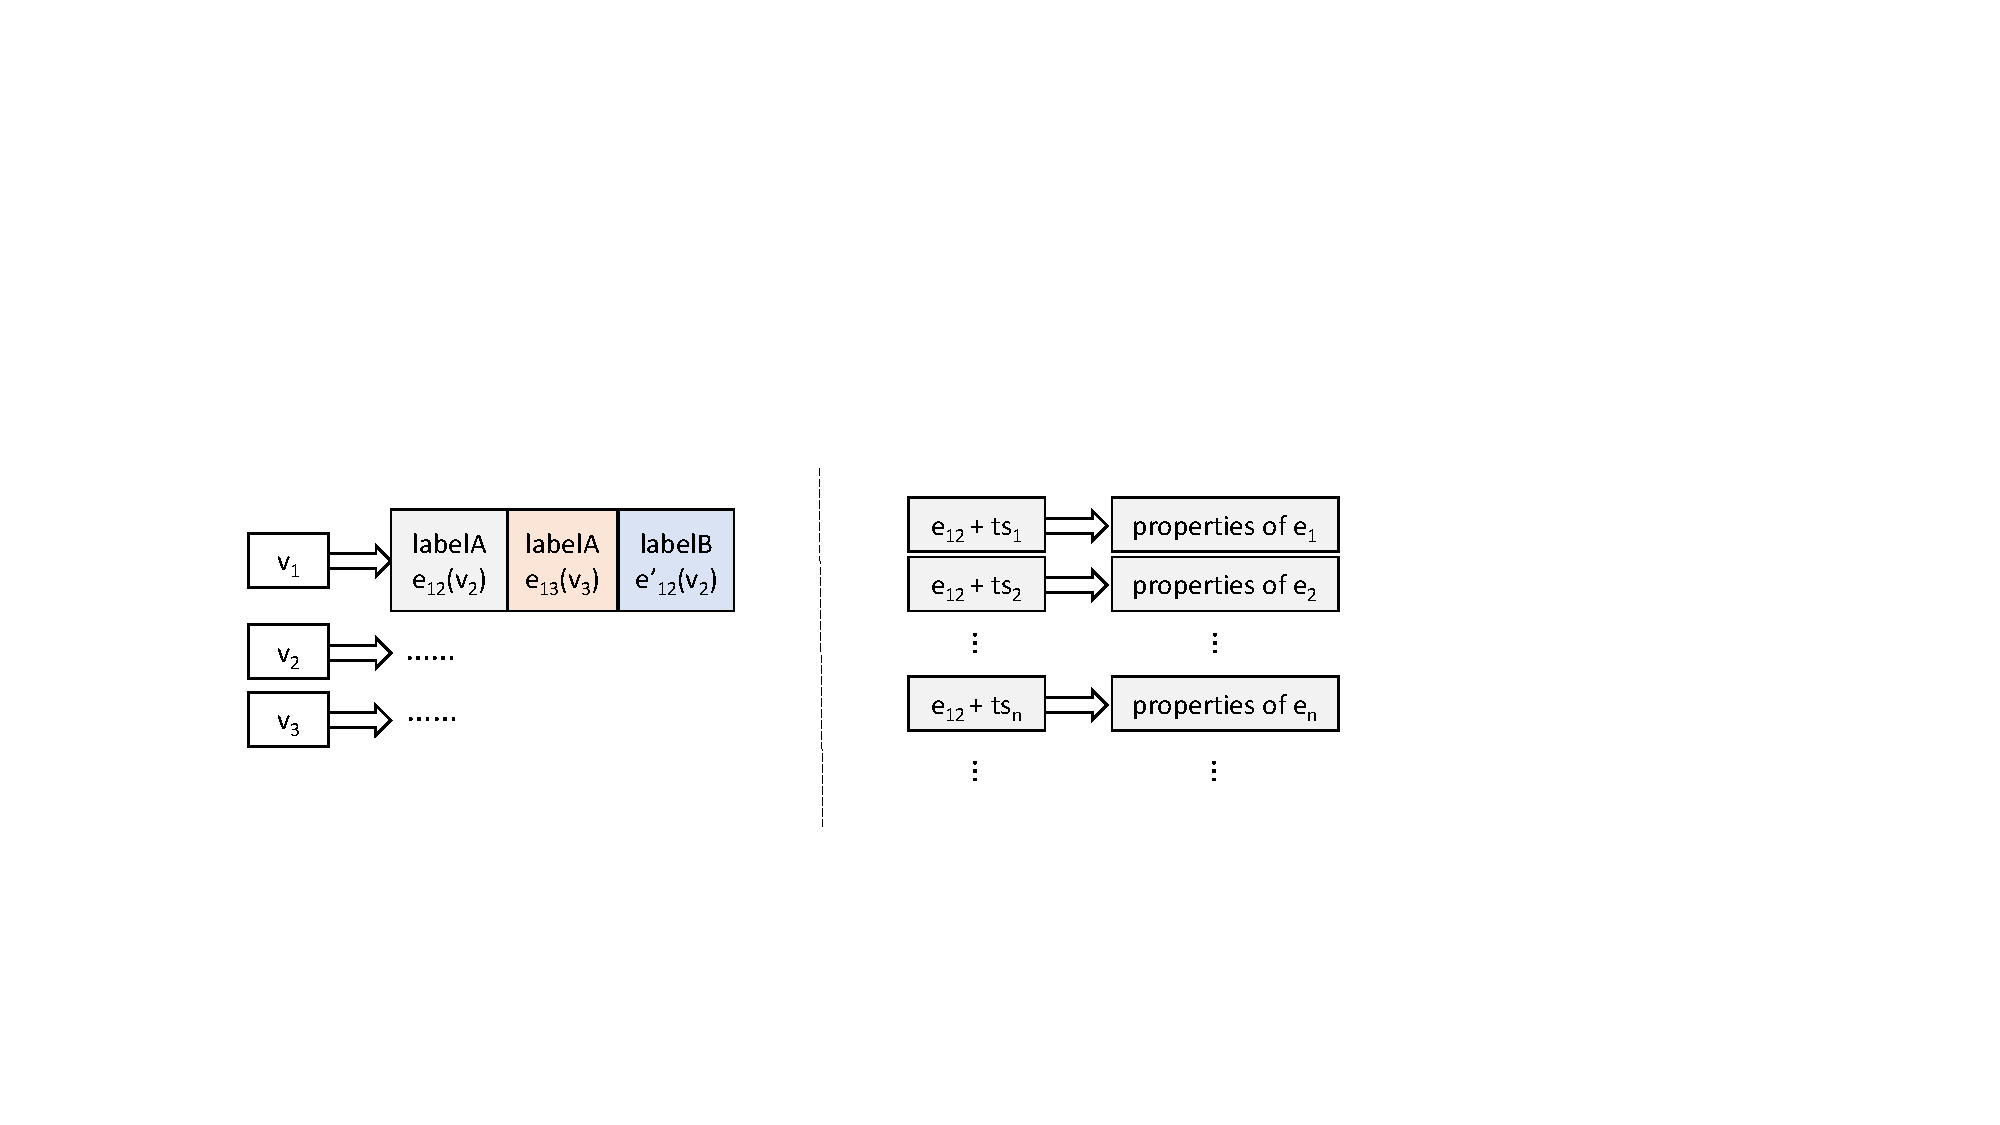
\includegraphics[width=150mm]{fig/curr_list.pdf}
\caption[HybriG在HBase中的数据表]{HybriG在HBase中的数据表分为两张,左边为Titan转化成的数据表,右边为边表。当属性图富含重边时,Titan数据表不被影响,边表将是一张高而窄的表。}
\label{fig:curr_list}
\end{figure}

为了解释HybriG在图查询上的优势,图\ref{fig:curr_list}展示了HybriG在HBase中的表结构,包括Titan自身的HBase数据表和HybriG特殊设计的边表。当属性图的重边数量爆炸性增长时,Titan的数据表并不会被影响,因为两点间同label的边至多只会存在一条,每个点的邻接表列数仍为不同label邻接的点数。另外,Titan中的边只存放统计信息,因此每个单元格(即每条边)的数据量实际很小。面对含有大量重边的属性图,各点的邻接表仍保持了列数和数据量上的精简。即使面对邻域点集查询的全表扫描,也能提供优异的性能。

另一方面,得益于邻接表的精简,Titan的缓存因此可以存放更多点集数据。对于邻域点集相关查询,如多跳邻域(k-hop)查询、路径查询、局部聚集系数计算等,具体的实现往往由多个基本的邻域点集查询组成,缓存的命中率就显得尤为重要。传统的解决方案中使用Titan存储所有的重边,使得缓存中只能存储少量点集的数据,大部分空间被边集数据占据,而具体的边集数据在查询中并不相关。在HybriG架构中,Titan的缓存能充分保留更多的点集数据,从而进一步提高邻域点集相关查询的缓存命中率。
综上,HybriG对邻域点集相关的查询具有很好的表现,后续的实验结果将展示具体的数据。

\subsubsection{边集相关查询的优势}
在许多刑侦推演场景中,往往只需要查询两点间拥是否拥有某种label的边,而不需要查看具体各个重边的数据。比如得知两人之间有共同住宿酒店的边相连后,基本可以断定两人认识,领域专家可以在图中继续推演出其他相关的人,后续有需要再展开这条关系,查看具体的各条酒店住宿记录。HybriG架构为这种场景提供了便利,上述场景相当于在HybriG架构的Titan图中进行游走(Graph traversal),当有需要时再展开某条边,在HBase边表中读回相应的边数据。

对于边集数据的读取,HybriG将所有边的数据存储在HBase边表中,而且每条边占一行,这使得对边的检索是行级别的检索,即在表中查找一行。传统的解决方案将重边数据都存储在Titan中,边集数据存储于各点的邻接表,而每个点的邻接表在HBase 数据表中占据一行,因此对边的检索是选定行后的列级别检索。HBase中行级别的检索要略优于列级别的检索,因此HybriG会略占优势。然而,HybriG对边的检索需要跨Titan 和 HBase 两个系统,会多一次交互的开销。实验表明,这两方面功过相抵,HybriG的边集数据查询性能与Titan相差不大。

HybriG架构在边集统计信息的查询或计算上会有很大优势。在HybriG架构中,Titan中某种label的边存在,代表原属性图中两点间拥有该label的边,具体的重边数据存储在HBase中的边表,而Titan中的边上的则存储了该label声明时设定的统计信息,如具体的重边数目、边上某个属性的最大最小值等。对于这些统计信息,可以直接在Titan中查询得到结果。


\section{Data Loader}
Data Loder模块负责图数据的导入,包括点的导入和边的导入。在HybriG架构中,点集数据都存储在Titan中,故点集数据导入直接在Titan上完成。边集数据虽然存储在HBase中,但Titan中的对应边上存储了重边的统计信息,因此需要同时更新Titan 和 HBase,以保证二者数据的一致。下面详述边的数据导入,以及如何保证Titan和HBase的数据一致性。

\subsection{边数据的高效导入}
在HybriG架构中,边的插入既要更新Titan,又要更新HBase中的边表。对于给定label的一条边数据,首先要查看Titan中两点间是否已有一条边表示这样的关系存在。若这样的边不存在,则将其创建。然后更新Titan边上的统计信息,再利用其边id将具体边的数据存入HBase中。算法\ref{alg:insert_one_edge}展示了上述逻辑。第1行查询Titan中该label的边,由于至多只有一条,故可用limit(1)加速。第2-4行若这样的边不存在,则在Titan中添加一条边。第5行根据要插入的边数据来更新Titan中边上的统计信息。第6行提交对Titan的所有修改。第7行将边数据写入HBase边表中,行键为e.id拼接上边的主键。
\begin{algorithm}
\caption{插入一条边的伪代码}
\label{alg:insert_one_edge}
\begin{algorithmic}[1] % 每1行显示一个行号
\REQUIRE Titan图接口graph,HBase边表接口hbaseTable,点v1,点v2,edgeLabel,边数据realEdge

\STATE e = v1.query().adjacent(v2).label(edgeLabel).limit(1).edges().next()
\IF{e == null}
\STATE {e = v1.addEdge(v2, edgeLabel)}
\ENDIF
\STATE updateStats(e, realEdge.properties)
\STATE graph.commit()
\STATE hbaseTable.put(e.id + realEdge.primaryKey, realEdge.properties)
\end{algorithmic}
\end{algorithm}

传统的解决方案将所有重边存储在Titan中,边数据的导入逻辑只需要上述代码的第3、5、6行。HybriG架构中每条边的插入多加了一次查询操作(第1行),以及HBase边表的插入操作(第7行),带来了额外的时间开销。而且最耗时的也是这两步操作,分别要从底层存储读取数据以及持久化所有修改到底层存储中。如果有批量重边需要导入,这些开销可以让所有重边来平摊,即在数据导入时,对于两点间同label的重边作为一批来处理,这样就可以共享查询操作的结果,对Titan边上统计信息更新的持久化操作(commit)也只需进行一次。批量导入重边数据的伪代码如算法\ref{alg:insert_batch_edges}所示。
\begin{algorithm}
\caption{重边数据的批量导入}
\label{alg:insert_batch_edges}
\begin{algorithmic}[1] % 每1行显示一个行号
\REQUIRE Titan图接口graph,HBase边表接口hbaseTable,点v1,点v2,edgeLabel,重边数据集allRealEdges

\STATE v1.query().adjacent(v2).label(edgeLabel).limit(1).edges().next()
\IF{e == null}
\STATE e = v1.addEdge(v2, edgeLabel)
\ENDIF
\FOR {realEdge in allRealEdges}
\STATE {updateStats(e, realEdge.properties)}
\ENDFOR
\STATE graph.commit()
\FOR {edge in allRealEdges}
\STATE {hbaseTable.put(e.id + realEdge.primaryKey, realEdge.properties)}
\ENDFOR
\end{algorithmic}
\end{algorithm}

在算法\ref{alg:insert_batch_edges}中,第1到8行是对Titan的更新,将两点间同label的重边作为一批处理,共享了对Titan的操作,从而平摊了额外的开销。另外第9到11行是对HBase边表的多次put操作,可以使用HBase的Bulk Loading 技术来进行加速。

\subsection{数据一致性}
在Titan的接口设计中,对图(graph)的初次操作将自动打开一个事务,执行 graph.commit() 时该事务提交,将事务里的修改持久化到底层存储中,Titan的事务保证了自身数据的一致性。HybriG架构由于把边数据的存储分开在Titan 和 HBase上,需要保证Titan和HBase上数据的一致性。比如Titan上关于重边的统计信息跟HBase边表的一致性,或者HBase边表里各行行键的边id部分跟Titan里的一致性。由于实现强一致性的代价过高,本架构保证的是Titan和HBase数据的最终一致性\supercite{eventually_consistent},即系统保证在经过错误恢复后,数据最终会达到一致的状态。最终一致性足以满足应用场景的需求。

由于只有边集数据是跨Titan和HBase存储的,下面讨论的都是边数据的导入。图\ref{fig:insert_steps}演示了边数据导入的三个步骤,第①步对应前述算法3中的第1~7行,更新Titan数据;第②步对应第8行,提交修改;第③步对应第9~11行,利用边id将边数据插入HBase边表中。对数据的持久化修改是第②③步,数据会出现不一致的原因是②③并不是原子的。如果②成功但是③失败了,即成功持久化了对Titan数据的修改,但对HBase边表的修改却失败了,则两方的数据出现不一致。失败的原因是多种多样的,比如程序内存溢出(Out of Memory)、网络中断、硬件故障等。

\begin{figure}[htbp]
\centering
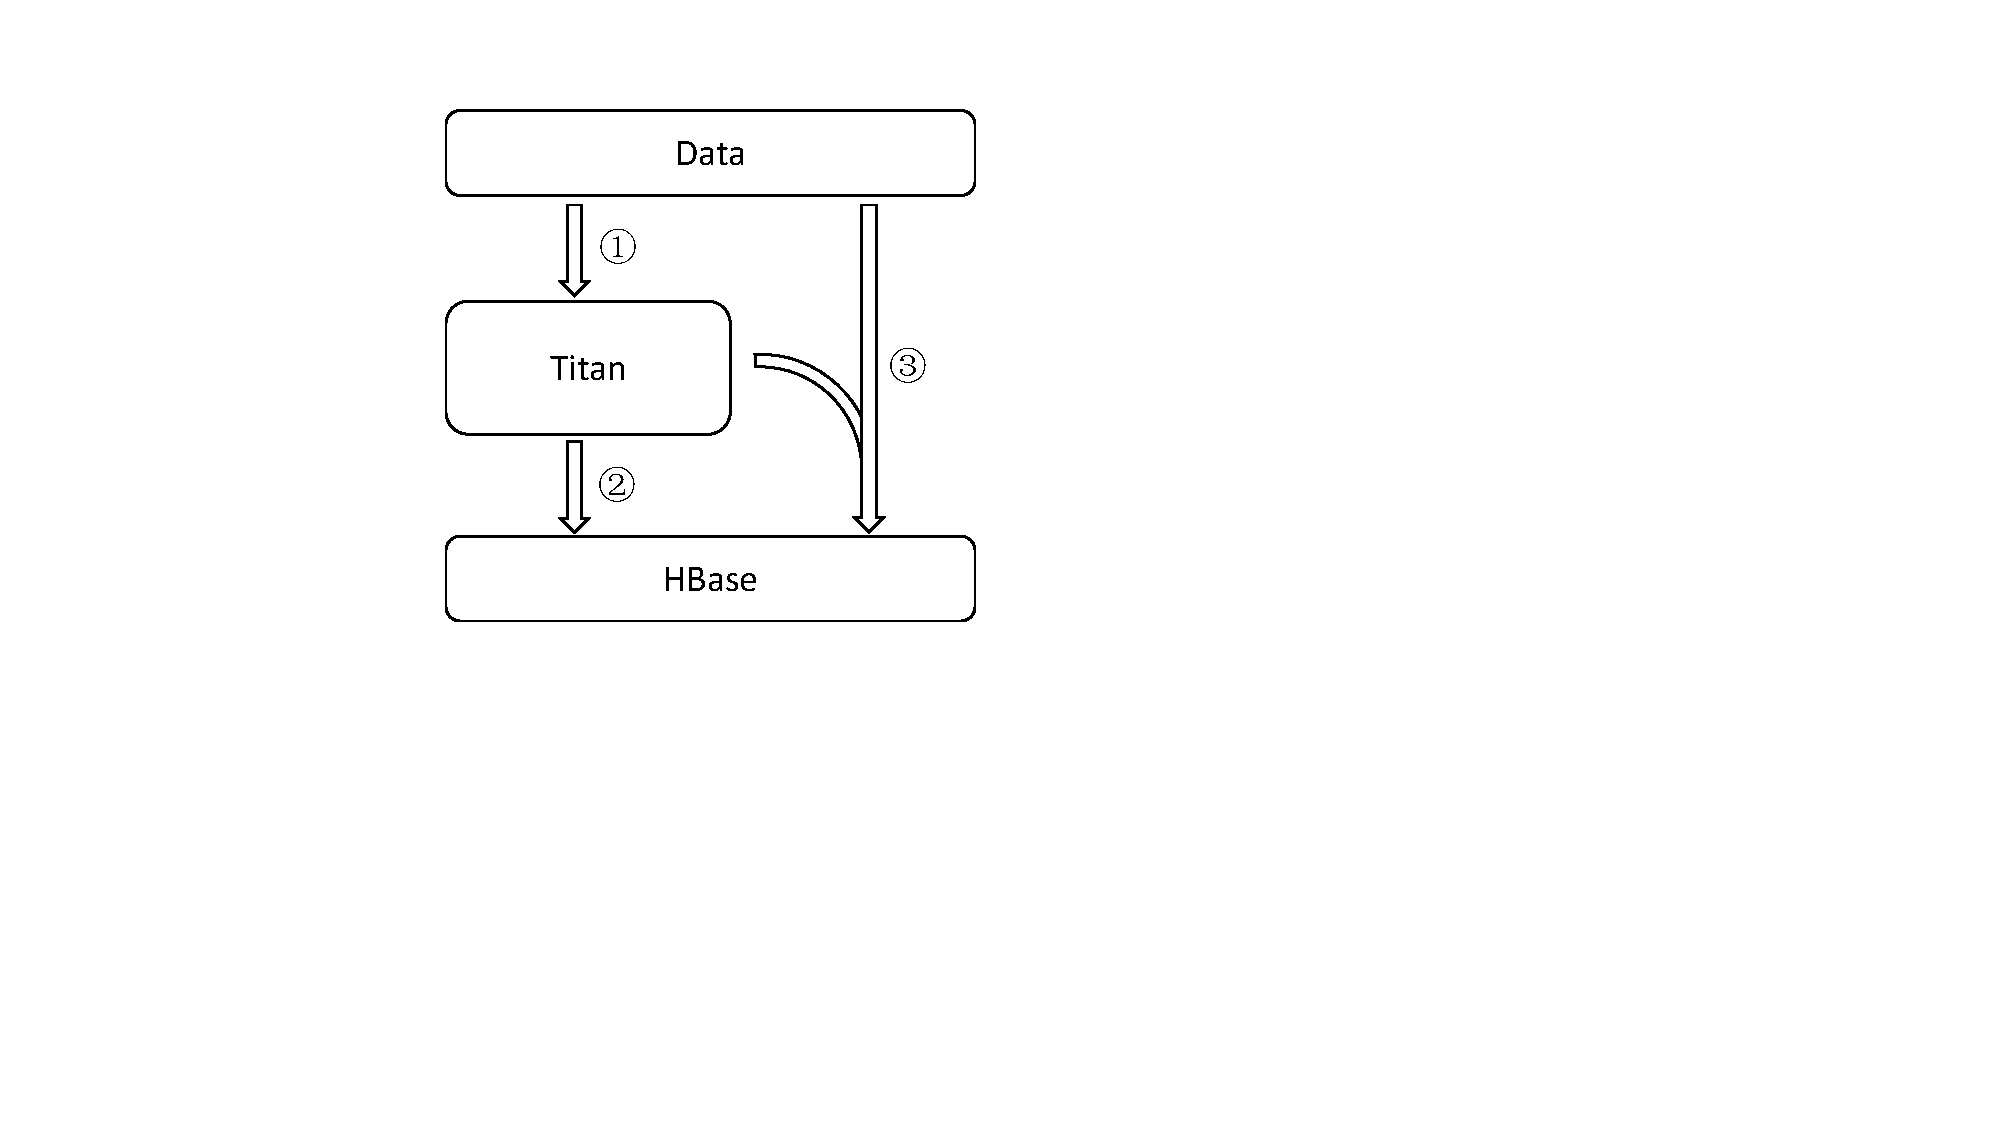
\includegraphics[width=60mm]{fig/insert_steps.pdf}
\caption[插入边数据的三个阶段]{边的数据导入分三步:①更新Titan数据;②提交Titan更改即graph.commit();③将数据插入HBase边表中}
\label{fig:insert_steps}
\end{figure}

当数据导入程序在故障之后重启时,这种不一致性需要被修复。该批次的边数据将会被重新导入,为了得知②是否已经成功,我们需要知道Titan中的数据是否已经被修改了。这可以利用Titan的
事务原子性来实现:在②提交之前,往Titan中写入一个成功标志(可以用一个点或属性来表示),然后再提交。根据原子性,该标志被成功写入当且仅当Titan的更新都被持久化。这样当数据导入程序重启时,我们先查看该标志是否存在,便可得知②是否已经成功了。若其已成功,则跳过这一步,直接进行第③步。该过程的伪代码如算法\ref{alg:consistence}所示。

\begin{algorithm}
\caption{保证一致性的边集数据批量导入}
\label{alg:consistence}
\begin{algorithmic}[1] % 每1行显示一个行号
\REQUIRE graph,batchID,HBase边表hbaseTable,点v1,点v2,edgeLabel,allRealEdges,所有边的属性
\STATE e = v1.query().adjacent(v2).label(edgeLabel).limit(1).edges().next()
\IF {hasNotCompleted(graph, batchID)}
	\IF {e == null}
		\STATE {e = v1.addEdge(v2, edgeLabel)}
	\ENDIF
	\FOR {realEdge in allRealEdges}
		\STATE {按需更新边上的统计信息}
	\ENDFOR
	\STATE markCompleted(graph, batchID)
	\STATE graph.commit()
\ENDIF
\FOR {edge in allRealEdges}
	\STATE {hbaseTable.put(e.id + edge.pk, properties)}
\ENDFOR
\end{algorithmic}
\end{algorithm}

算法\ref{alg:consistence}中,第2行的函数hasNotCompleted判断给定的Titan图中是否存在给定批次的成功标志。若不存在则执行第3到10行更新Titan,其中第9行的markCompleted函数在Titan图中插入该批次的成功标志。

值得一提的是,我们在HBase中并没有放置成功标志。如果数据导入程序在第③步成功插入HBase数据后出现故障,则重启后还会将边集数据再次插入HBase中。但这是没有问题的,因为HBase边表中的数据不存在统计信息,因此不存在更新操作,所有操作都是新数据的插入操作。我们设置HBase的最大版本数为1,则多次插入同一内容到一个单元格,实际只保存一份,不会增加存储开销。


% vim:ts=4:sw=4
